\chapter{Testing with All Data}
\label{sec:proper_vectorization}

In this section we will take what we have learned from the experiments in the previous sections and apply that knowledge to the original data set augmented with the additional data that we collected. The total category count tallies can be located in the Attachments in Table \ref{tab:data_counts}. These experiments will provide us with a better understanding of how the data is interacting with the active learning sampling strategies and the PWC classifier. We will also try removing some data from the set if the text length is below some threshold, evaluate the performance with a reduced number of categories, and explore the performance of xPAL using all available data.

\section{Classifier Evaluation Revisited}

We wanted to re-run the classifier experiment that we ran with the original data with the new data to get an idea of how the new data effected influenced the classifiers from Scikit-Learn. The results are shown in Table \ref{tab:best_errors_all_data}.

\begin{table}[ht]
    \centering
    \caption{Test errors for best performing classifiers using all data.}
    \begin{tabular}{lr}
\toprule
                     Model &  Error \\
\midrule
                 LinearSVC &  0.429 \\
Tensor Flow Neural Network &  0.433 \\
    K Neighbors Classifier &  0.471 \\
\bottomrule
\end{tabular}

    \label{tab:best_errors_all_data}
\end{table}

Its interesting to see that the errors increased across the board but our previous results could have been skewed possibly because we had so few data samples in some categories. We ran the Bagging Classifier GridSearchCV from the previous chapter and again could not tune the model to perform better than the base untuned LinearSVC.

\section{Active Learning using All Data}

In these experiments we tested all the active learning methods with the corrected TF-IDF vectorizer transformation. Instead of incorrectly vectorizing the data then importing the matrix to be used with \cite{kottke2021toward} probablistic active learning code, we exported the raw text data and then split the text data, fit and transformed the vectorizer to the train data, then transformed the test data and conducted our experiments with the modified code. In Figure \ref{fig:probal_original_proper_vect} we re-ran a previous experiment using just the original data so we could have a more accurate comparison with the results for all the data shown in Figure \ref{fig:probal_all_proper_vect}. In Figures \ref{fig:probal_original_proper_vect_50_st_filter} and \ref{fig:probal_all_proper_vect_50_st_filter} we used an arbitrary text length filter of 50 characters to see how the performance of the selection strategies changed when we removed some of the data. The categorical data splits for the 50 character filter can be found in the Attachments in Table \ref{tab:50_char_filter_data_counts}.

\begin{figure}[ht]
    \centering
    \begin{subfigure}{0.49\textwidth}
        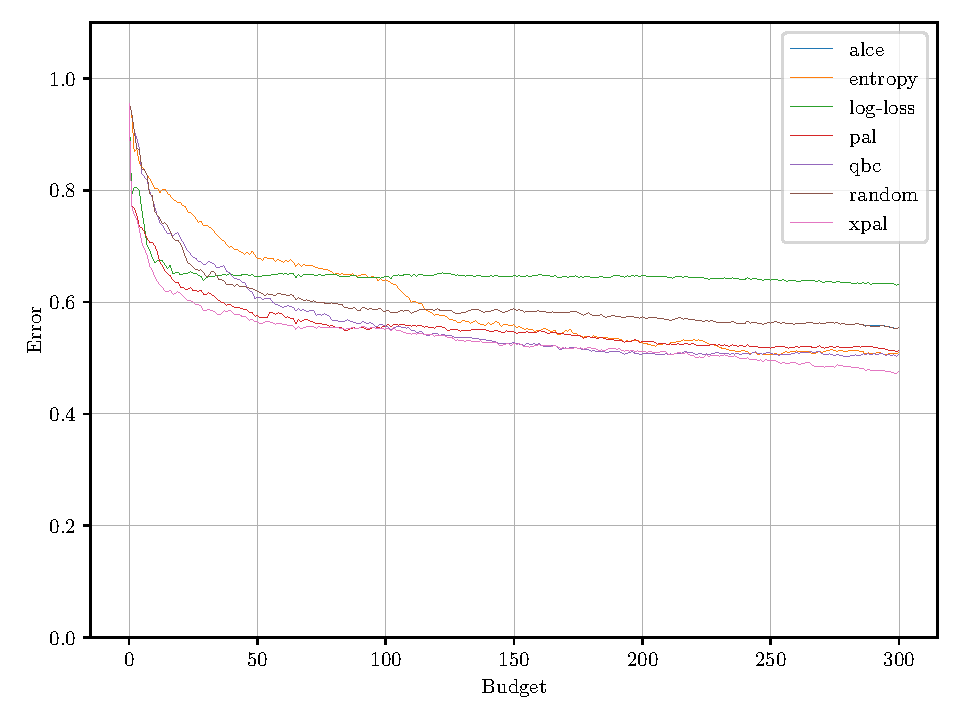
\includegraphics[width=\textwidth]{../img/plot_text_data_original_proper_vectorizer_test_results.pdf}
        \caption{No text length filter and proper vectorization.}
        \label{fig:probal_original_proper_vect}
    \end{subfigure}
    \hfill
    \begin{subfigure}{0.49\textwidth}
        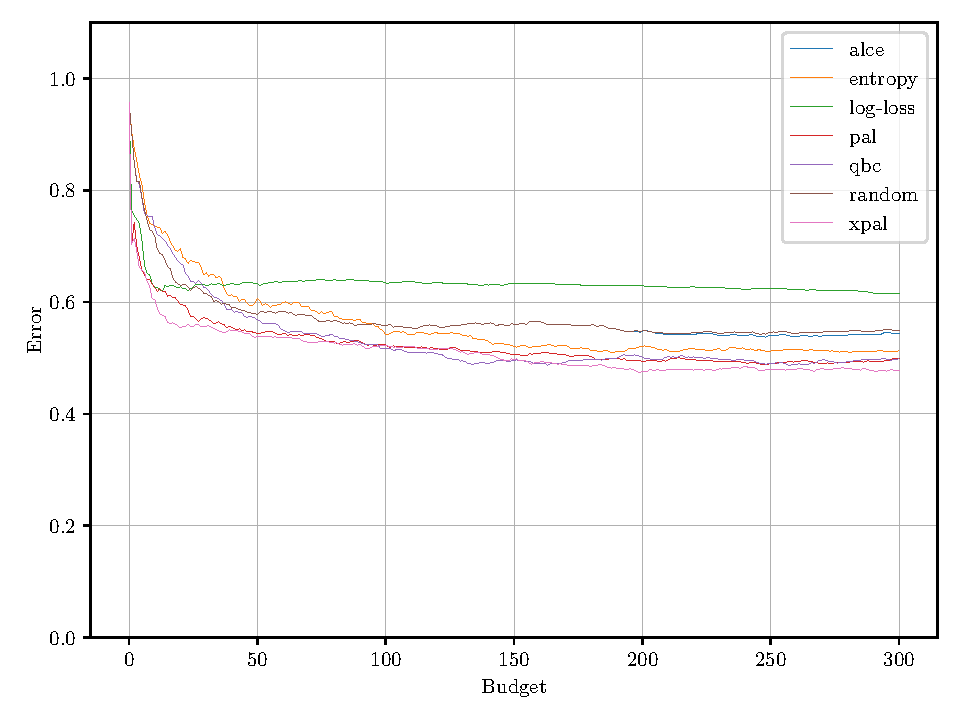
\includegraphics[width=\textwidth]{../img/plot_text_data_original_proper_vectorizer_50_st_filter_test_results.pdf}
        \caption{Text length data $>50$ and proper vectorization.}
        \label{fig:probal_original_proper_vect_50_st_filter}
    \end{subfigure}
    \caption{Active learning results using the original data.}
\end{figure}

We again used the different active learning methods and PWC with the Cosine kernel to run our experiments. We ran 10 test runs for each method and then averaged the test error of all the runs resulting in a single curve for each sampling strategy, exactly as we did previously. We only used the first 300 data points instead of using the entire budget because we have seen that the error plateaus and we want to reduce the amount of time it takes to run our experiments. As a result, the test error doesn't converge in these plots because we are only using a portion of the budget. With the original data we can see that the xPAL sampling strategy finds the best data early (20-30 budget range) in the sampling process and exploits this to improve the classifier the most. Eventually we see that PAL and QBC have similar performance to xPAL but, ultimately, after 300 samples xPAL is the best performing sampling strategy.

Using all the data, we repeated this same experiment and found that the selection strategies testing error results seemed to have a bit more separation. The results are shown in Figure \ref{fig:probal_all_proper_vect}. In both experiments in this section it appeared that the test error for xPAL was converging to around roughly 50\%. But for the second experiment using all the data xPAL was finding and exploiting the best data points earlier and for longer in the sampling process. We can see the dominance of xPAL throughout the plot except around the 200 budget range where entropy sampling starts to momentarily perform well.

\begin{figure}[ht]
    \centering
    \begin{subfigure}{0.49\textwidth}
        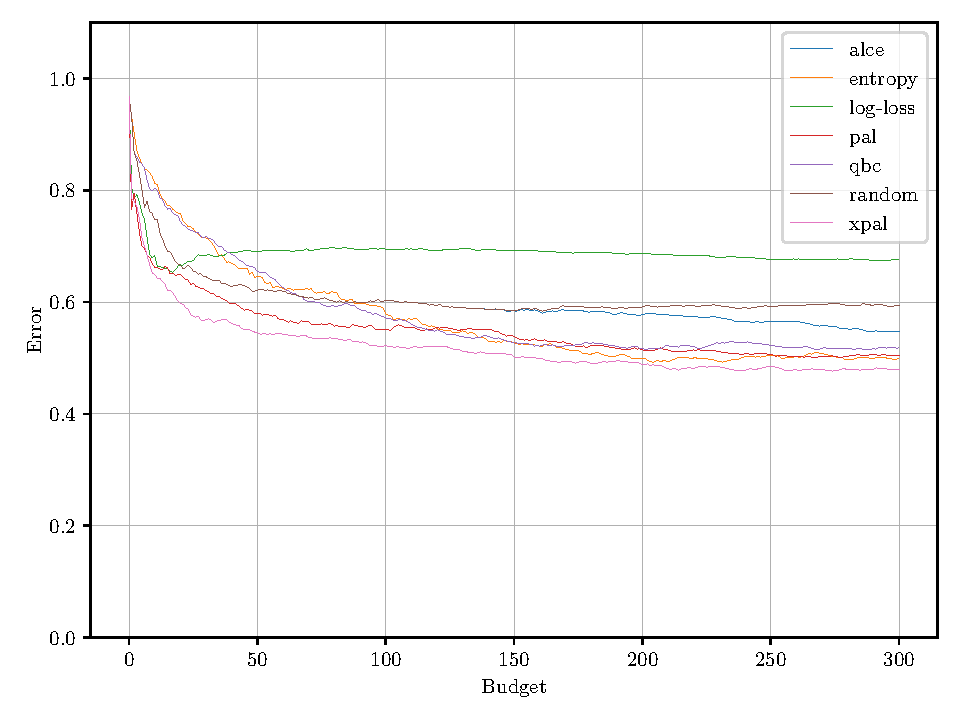
\includegraphics[width=\textwidth]{../img/plot_text_data_all_proper_vectorizer_test_results.pdf}
        \caption{No text length filter and proper vectorization.}
        \label{fig:probal_all_proper_vect}
    \end{subfigure}
    \hfill
    \begin{subfigure}{0.49\textwidth}
        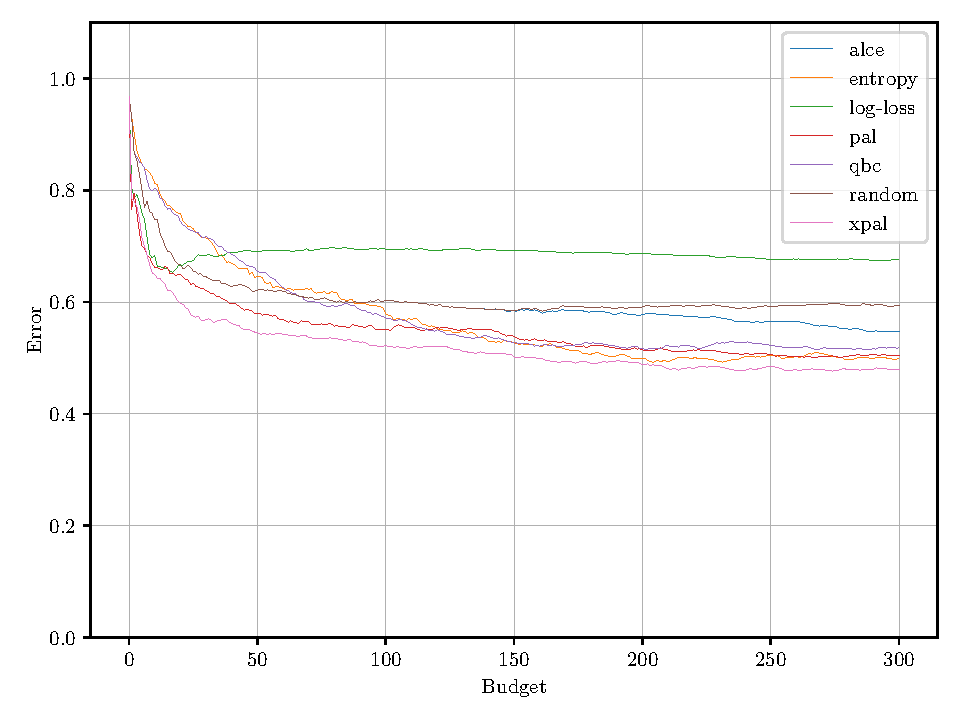
\includegraphics[width=\textwidth]{../img/plot_text_data_all_proper_vectorizer_50_st_filter_test_results.pdf}
        \caption{Text length data $>50$ and proper vectorization.}
        \label{fig:probal_all_proper_vect_50_st_filter}
    \end{subfigure}
    \caption{Active learning results using all data.}
\end{figure}

In both the re-run original data and all data experiments, xPAL appears to perform well an average over 10 different runs in comparison to the other selection strategies, it even seemed to perform markedly well with more data available and then having some filtering applied as shown in Figure \ref{fig:probal_all_proper_vect_50_st_filter} where its dominance over the other selection was even more apparent. This led us to believe that the more data that is available and the more text that is available per data sample the better xPAL will perform. This will not always be true but it seems that if we have a large enough amount of text, 50 characters being an arbitrary example, xPAL will have an easier time selecting the best data points to label.


We were curious what xPAL was doing when more data was available, so while running the experiments we recorded when a data point was selected (its index in the selection budget) and for which category it was selected from. This data is shown here in Figure \ref{fig:xpal_data_selection}.

\begin{figure}[ht]
  \centering
  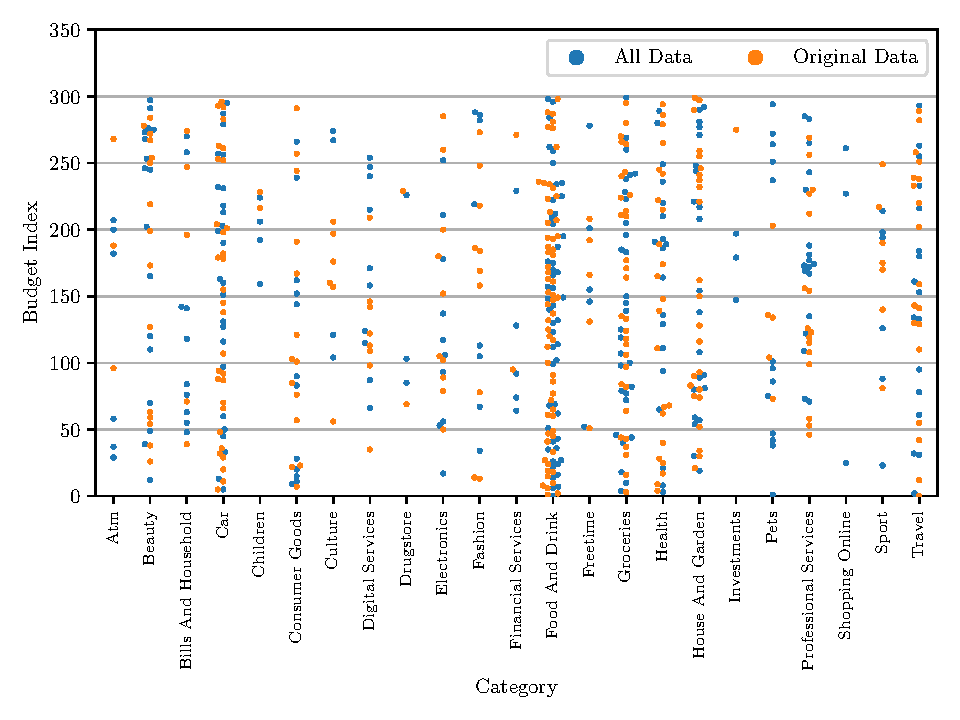
\includegraphics[width=\textwidth]{../img/plot_xpal_selection_dist.pdf}
  \caption{Data point selection swarm plot using xPAL.}
  \label{fig:xpal_data_selection}
\end{figure}

This distribution data is not averaged and is from a sample run for each of the data sets without any filtering. In this data split the 'Shopping Online' category for the original data went without asking for a label in the given budget window. It is interesting that it chose not to select its sole sample but intuitively it may make sense because there is only one other 'Online Shopping' sample point and it is in the test set. Its possible that because there is only one sample xPAL may not yet find it necessary to know its label this early in the budget and other data points labels are more valuable to know. It is clear from Figure \ref{fig:xpal_data_selection} that when new data is available the xPAL selection strategy reevaluates what is important and selects data points that are more likely to be helpful. This is a good sign that xPAL is able to adapt to the data and find the most helpful data points.

\section{LinearSVC with Text Length Filtering} 

We have some data that may not have enough text to classify correctly and others that have more than 1000 characters of text that may be noisy. We also know that sometimes while scraping the text data from a website we collected a non empty string that actually provided no words that were related to the label, such as a simple error or warning message.

However, using all available data, we now have the luxury of having more than the minimum of 2 data points in some categories and can afford to remove data from the set that may have unhelpful or confusing words in the text. We decided to explore if filtering the data based on text length could improve the performance of the classifier and use LinearSVC as it has performed well with this data previously and it is relatively fast to train.

Before conducting the filtering data experiments we can view how the text length is distributed throughout our preprocessed and scrubbed text data as shown in Figure \ref{fig:string_length_dist}. This can help us visualize how much data we may be removing if we filter the data based on text length.

% \begin{figure}[ht]
%     \centering
%     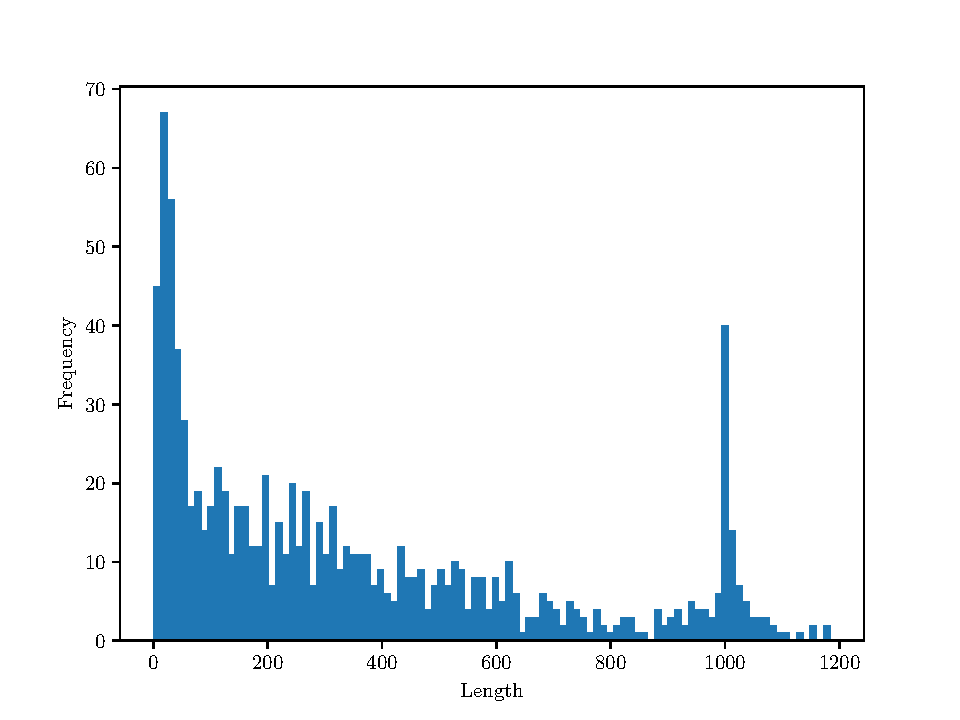
\includegraphics[width=\scale\textwidth]{../img/plot_string_length_dist_all_data.pdf}
%     \caption{Distribution of text length for all data in 100 bins.}
%     \label{fig:string_length_dist}
% \end{figure}

\begin{figure}[ht]
    \centering
    \begin{subfigure}{0.49\textwidth}
        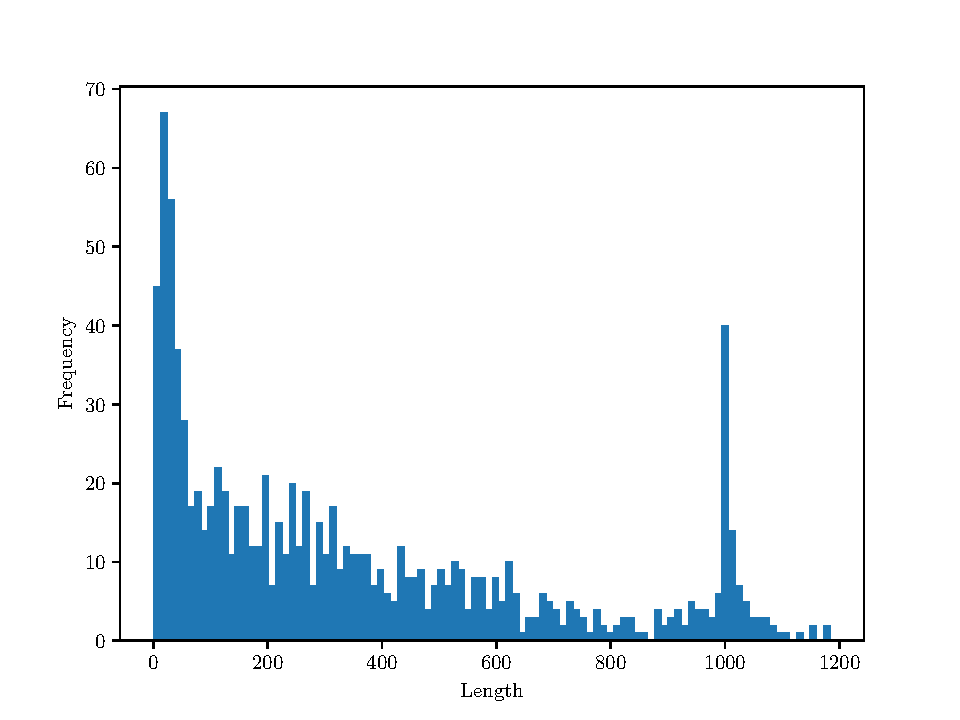
\includegraphics[width=\textwidth]{../img/plot_string_length_dist_all_data.pdf}
        \caption{Distribution of text length for all data in 100 bins.}
        \label{fig:string_length_dist}
    \end{subfigure}
    \hfill
    \begin{subfigure}{0.49\textwidth}
        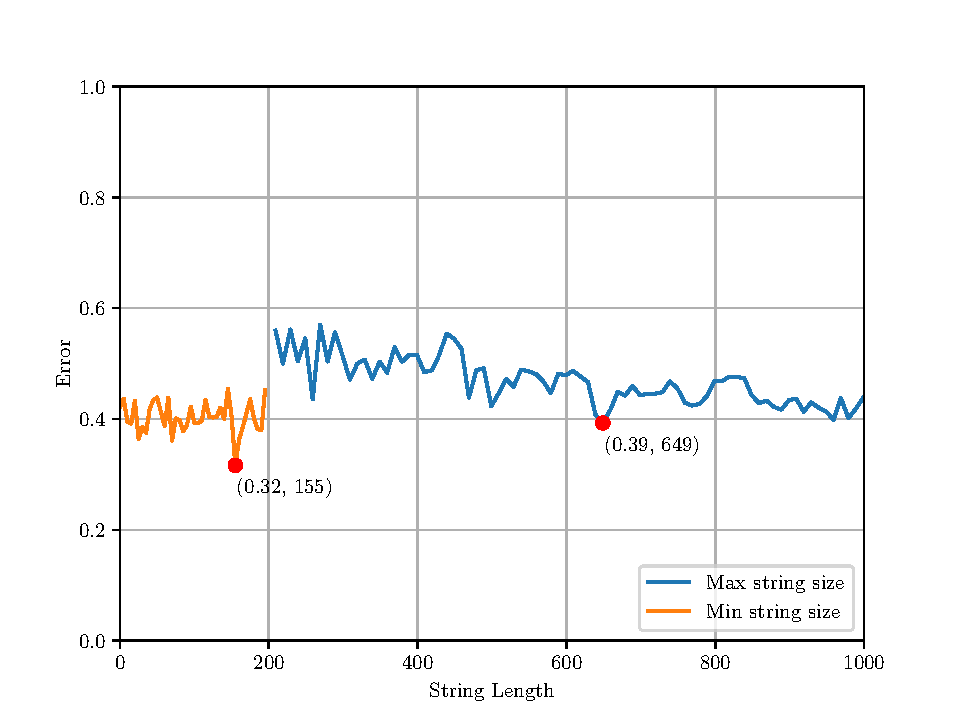
\includegraphics[width=\textwidth]{../img/plot_data_length_grid_search.pdf}
        \caption{Test error results for best LinearSVC with varying text length requirements.}
        \label{fig:grid_search_text_length}
    \end{subfigure}
    \caption{Text length experiments data and results.}
\end{figure}

The distribution of the text show a steady decrease in length and frequency until around the 850 length mark where we have an increase of data with large amounts of text. The spike here is a results from when we capped the non English data text to 1000 characters so that we could translate all of our data using the Azure translation services.

We imported the data and either selected a minimum number of characters or we altered the maximum number of characters allowed and created a new dataset. For each run we selected the data based on this criteria and then built the TF-IDF array. For the minimum string size tests we incremented the string size by 1 character. While for the max string size tests we decremented the string size by 10. We again used a train test split of 25\% which has been our standard for testing throughout our experiments. We found that around the 200 character mark we would filter out too much data and would not have a minimum representation (2 data points) for all the categories. The results for this experiment are shown in Figure \ref{fig:grid_search_text_length}.

% \begin{figure}[ht]
%     \centering
%     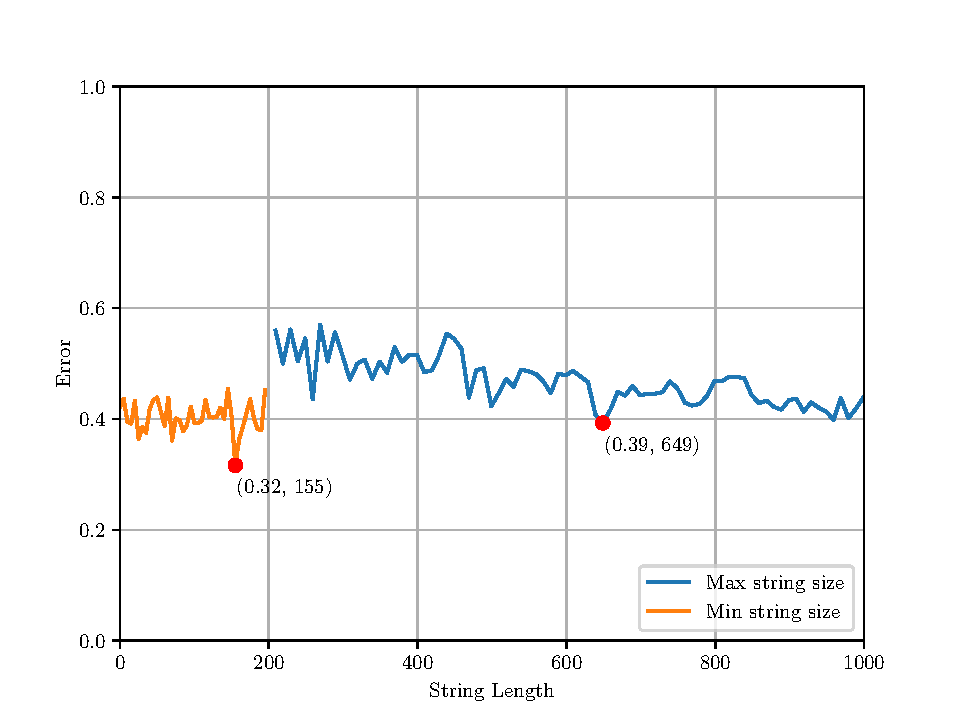
\includegraphics[width=\scale\textwidth]{../img/plot_data_length_grid_search.pdf}
%     \caption{Test error results for best LinearSVC with varying text length parameters.}
%     \label{fig:grid_search_text_length}
%   \end{figure}

We also tested with a minimum text length and a maximum text length constraint implemented together but this combination did not yield any obvious gains. This naive approach to filtering the data did not yield any obvious improvements in the test error. At best it may have filtered out some bad data and provided a small improvement in the test error. However, when implementing xPAL we hope to have it filter out the bad data in a more calculated manner.

\section{Testing with Fewer Categories}

In this section we will briefly look at the PWC with xPAL and LinearSVC performance using progressively fewer categories. We will use all available data and remove the category from the data set if it has less than the minimum number of samples. We assume that reducing the number of categories decreases the test error. Intuitively, this should be the case because as we reduce the number of categories we are reducing the number of classes that the classifier has to learn and classify. This should make the classification task easier and therefore the test error should decrease. However, we have a lot of data in the 'Food and Drink' and 'Groceries' categories and we have seen that the classifiers struggle to classify these categories correctly. Results from some tests are shown for the PWC with xPAL in Figure \ref{fig:all_data_category_reduction_xpal}.

\begin{figure}[ht]
    \centering
    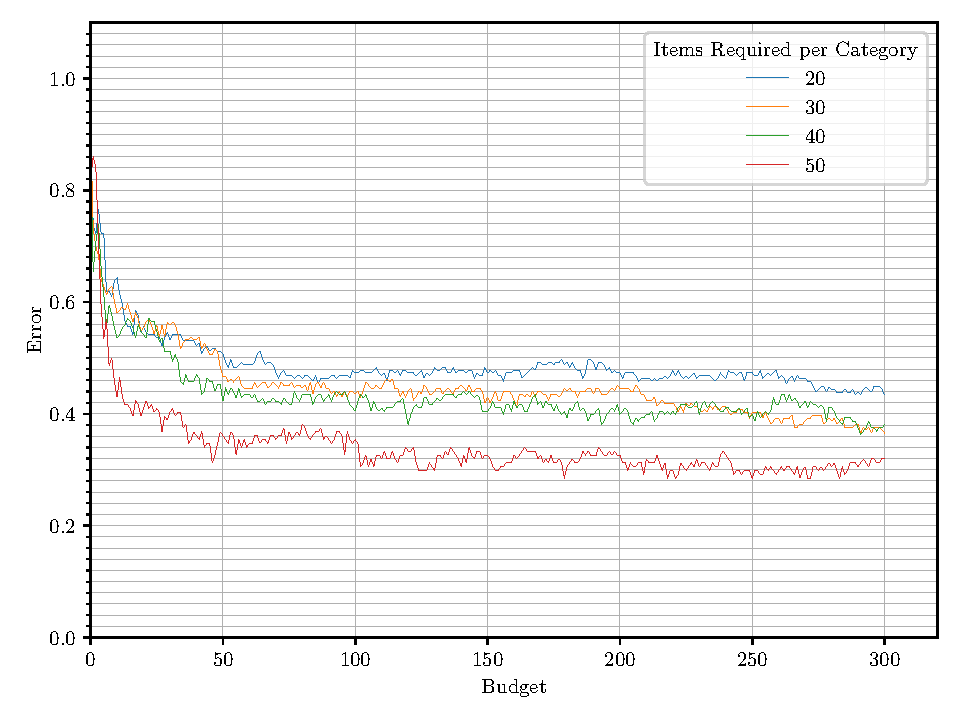
\includegraphics[width=\scale\textwidth]{../img/plot_text_data_all_category_reduction_test_results.pdf}
    \caption{PWC with xPAL with category reduction on all data.}
    \label{fig:all_data_category_reduction_xpal}
\end{figure}

\cite{dumais2000hierarchical} discusses the issue of reducing the number of categories in web content classification in their paper. They note that reducing the number of categories can improve the accuracy and efficiency of the model by reducing the complexity of the classification problem. However, they also note that reducing the number of categories can reduce the specificity of the classification and make it more difficult to distinguish between similar categories.

Looking at the results from the xPAL and PWC tests in Table \ref{fig:all_data_category_reduction_xpal} we can see that we have generally have reduction in test error except between the 30 and 40 category minimum tests. This table also shows us the categories that were used in the classification. This might tell us that 'Consumer Goods', 'House and Garden', and 'Professional Services' are easily linearly as the change in test error after 300 samples was small.

Reviewing these results it seems that 'Food and Drink' and 'Groceries' may be skewing a portion of the test error and if there was better way to classify these categories it would improve the overall test error.

\begin{table}[ht]
     \centering  
     \caption{LinearSVC performance with category reduction on all data, where category minimum is the min number of samples required.}
     \begin{tabular}{p{2cm}|p{1.8cm}|p{7.5cm}|p{1.4cm}}
\toprule
 Category Minimum &    Error &                                                                                                                              Categories &  Count \\
\midrule
               20 & 0.359756 & [Beauty, Car, Consumer Goods, Fashion, Food And Drink, Groceries, Health, House And Garden, Pets, Professional Services, Sport, Travel] &     12 \\
               30 & 0.362416 &                       [Beauty, Car, Consumer Goods, Food And Drink, Groceries, Health, House And Garden, Professional Services, Travel] &      9 \\
               40 & 0.320896 &                                                              [Beauty, Car, Food And Drink, Groceries, Health, House And Garden, Travel] &      7 \\
               50 & 0.234783 &                                                                                        [Car, Food And Drink, Groceries, Health, Travel] &      5 \\
\bottomrule
\end{tabular}

     \label{tab:lscv_all_data_category_reduction} 
\end{table}

We ran this experiment again to see if we could increase the performance by taking 'Groceries' completely out of the equation. The results are shown here and the categories are the same as previously with the only difference being that 'Groceries' is not included in the test.

\begin{table}[ht]
    \centering  
    \caption{Same as previous table but with 'Groceries' category removed.}
    \begin{tabular}{p{2cm}|p{1.8cm}|p{1.4cm}}
\toprule
 Category Minimum &    Error  &  Count \\
\midrule
               20 & 0.278912 &     11 \\
               30 & 0.303030 &      8 \\
               40 & 0.279661 &       6 \\
               50 & 0.214286  &      4 \\
\bottomrule
\end{tabular}

    \label{tab:lscv_category_reduction_no_groceries} 
\end{table}

It is interesting to see how removing the 'Groceries' category was able to improve the test error across the board. It may be that since we have removed a category with similar data to 'Food and Drink' the classifier is able to better classify the 'Food and Drink' category and because we have a lot of data in this category we perform better. 

\begin{table}[ht]
    \centering  
    \caption{Same as previous table but with 'Food and Drink' category removed.}
    \begin{tabular}{p{2cm}|p{1.8cm}|p{1.4cm}}
\toprule
 Category Minimum &    Error  &  Count \\
\midrule
               20 & 0.423423 &     11 \\
               30 & 0.343750 &      8 \\
               40 & 0.256098 &      6 \\
               50 & 0.190476 &      4 \\
\bottomrule
\end{tabular}

    \label{tab:lscv_category_reduction_no_food} 
\end{table}

Removing the 'Food and Drink' category did not have the same effect as removing the 'Groceries' category. This may be because the 'Food and Drink' category, again, has a lot of data and removing it may have reduced the amount of data available for the classifier to learn from.